% questions.tex —— 2003 年·北京卷·文科 · 题目内容片段（无答案）
% 由 tools/generate_projects.py 依来源总账自 2003/2003_数学真题_北京文_试题.md 生成，勿手改（改源 MD 后重跑）


\begin{gktip}
\textbf{来源说明}：本稿按固定候选 PDF 第 1–2 页逐题转录，原卷印刷页码 126–127。来源发布者、版次、复制/扫描链及官方身份未核。固定 PDF 仅含题面，无答案或评分页，官方答案字段为 null。
\textbf{题号范围}：原页可见 Q1–Q20；本候选 PDF 未见 Q21、Q22，不从其他版本补题。
\textbf{待核保留}：Q18 原题文字与图示顶点字母不统一，忠实保留原字并在题下标记；不据图示静默改名。
\end{gktip}

\gkpart{一、选择题}

\begin{question}
\gkti{1}
设集合 \(A=\{x\mid x^2-1>0\}\)，\(B=\{x\mid \log_2x>0\}\)，\(A\cap B\) 等于（　）

    (A) \(\{x\mid x>1\}\)
    (B) \(\{x\mid x>0\}\)
    (C) \(\{x\mid x<-1\}\)
    (D) \(\{x\mid x<-1\text{ 或 }x>1\}\)

\end{question}
\begin{question}
\gkti{2}
设 \(y_1=4^{0.9}\)，\(y_2=8^{0.44}\)，\(y_3=\left(\frac12\right)^{-1.5}\)，则（　）

    (A) \(y_3>y_1>y_2\)
    (B) \(y_2>y_1>y_3\)
    (C) \(y_1>y_2>y_3\)
    (D) \(y_1>y_3>y_2\)

\end{question}
\begin{question}
\gkti{3}
“\(\cos 2\alpha=-\frac{\sqrt3}{2}\)”是“\(\alpha=k\pi+\frac{5\pi}{12},\ k\in\mathbb Z\)”的（　）

    (A) 必要非充分条件
    (B) 充分非必要条件
    (C) 充分必要条件
    (D) 既非充分又非必要条件

\end{question}
\begin{question}
\gkti{4}
已知 \(\alpha,\beta\) 是平面，\(m,n\) 是直线。下列命题中不正确的是（　）

    (A) 若 \(m\parallel n\)，\(m\perp\alpha\)，则 \(n\perp\alpha\)
    (B) 若 \(m\parallel\alpha\)，\(\alpha\cap\beta=n\)，则 \(m\parallel n\)
    (C) 若 \(m\perp\alpha\)，\(m\perp\beta\)，则 \(\alpha\parallel\beta\)
    (D) 若 \(m\perp\alpha\)，\(m\subset\beta\)，则 \(\alpha\perp\beta\)

\Needspace{0.4\textheight}
\end{question}
\begin{question}
\gkti{5}
如图，直线 \(l:x-2y+2=0\) 过椭圆的左焦点 \(F_1\) 和一个顶点 \(B\)，该椭圆的离心率是（　）

    (A) \(\frac15\)
    (B) \(\frac25\)
    (C) \(\frac{\sqrt5}{5}\)
    (D) \(\frac{2\sqrt5}{5}\)
\nopagebreak[4]
\begin{center}% Generator: hand-authored TikZ schematic traced from the fixed source; curve and coordinates are illustrative.
% Source ID: src-dcc6a2c21c7b8e7b8f23f5188f34d7f542f94e40f4219b54cfb85a0d7004bc0f
% PDF SHA-256: 7fc0fd289fc486a0ae1c16a9ab5b4f0561830897df6e8897c50666f03d511913
% PDF page 1; printed page 126; question 5.
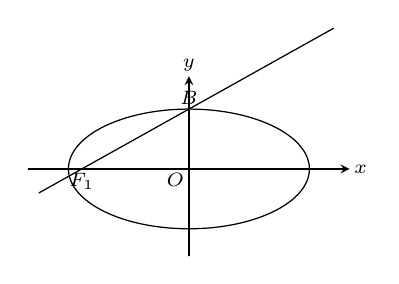
\begin{tikzpicture}[
  x=0.68cm,y=0.76cm,line width=0.45pt,line cap=round,>=stealth,
  every node/.style={font=\scriptsize,inner sep=1.5pt}
]
  \draw[->] (-3.0,0)--(3.0,0) node[right] {$x$};
  \draw[->] (0,-1.45)--(0,1.55) node[above] {$y$};
  \draw (0,0) ellipse [x radius=2.25,y radius=1.0];
  \draw (-2.8,-0.4)--(2.7,2.35);

  \node[below left] at (0,0) {$O$};
  \node[above] at (0,1) {$B$};
  \node[below] at (-2,0) {$F_1$};
\end{tikzpicture}
\end{center}
\nopagebreak[4]
\end{question}
\begin{question}
\gkti{6}
若 \(z\in\mathbb C\) 且 \(|z+2-2i|=1\)，则 \(|z-2-2i|\) 的最小值是（　）

    (A) 2
    (B) 3
    (C) 4
    (D) 5

\end{question}
\begin{question}
\gkti{7}
如果圆台的母线与底面成 \(60^\circ\) 角，那么这个圆台的侧面积与轴截面面积的比为（　）

    (A) \(2\pi\)
    (B) \(\frac32\pi\)
    (C) \(\frac{2\sqrt3}{3}\pi\)
    (D) \(\frac12\pi\)

\end{question}
\begin{question}
\gkti{8}
\Needspace{5\baselineskip}
若数列 \(\{a_n\}\) 的通项公式是
\nopagebreak[4]
\[
a_n=\frac{3^{-n}+(-1)^n3^{-n}}2,\quad n=1,2,\ldots,
\]
则 \(\displaystyle\lim_{n\to\infty}(a_1+a_2+\cdots+a_n)\) 等于（　）

    (A) \(\frac1{24}\)
    (B) \(\frac18\)
    (C) \(\frac16\)
    (D) \(\frac12\)

\end{question}
\begin{question}
\gkti{9}
从黄瓜、白菜、油菜、扁豆 4 种蔬菜品种中选出 3 种，分别种在不同土质的三块土地上，其中黄瓜必须种植，不同的种植方法共有（　）

    (A) 24 种
    (B) 18 种
    (C) 12 种
    (D) 6 种

\end{question}
\begin{question}
\gkti{10}
\Needspace{5\baselineskip}
某班试用电子投票系统选举班干部候选人。全班 \(k\) 名同学都有选举权和被选举权，他们的编号分别为 \(1,2,\ldots,k\)，规定：同意按“1”，不同意（含弃权）按“0”，令
\nopagebreak[4]
\[
a_{ij}=\begin{cases}
1,&\text{第 }i\text{ 号同学同意第 }j\text{ 号同学当选，}\\
0,&\text{第 }i\text{ 号同学不同意第 }j\text{ 号同学当选，}
\end{cases}
\]
其中 \(i=1,2,\ldots,k\)，且 \(j=1,2,\ldots,k\)，则同时同意第 1、2 号同学当选的人数为（　）

    (A) \(a_{11}+a_{12}+\cdots+a_{1k}+a_{21}+a_{22}+\cdots+a_{2k}\)
    (B) \(a_{11}+a_{21}+\cdots+a_{1k}+a_{12}+a_{22}+\cdots+a_{k2}\)
    (C) \(a_{11}a_{12}+a_{21}a_{22}+\cdots+a_{k1}a_{k2}\)
    (D) \(a_{11}a_{21}+a_{12}a_{22}+\cdots+a_{1k}a_{2k}\)

\end{question}
\gkpart{二、填空题}

\begin{question}
\gkti{11}
已知某球体的体积与其表面积的数值相等，则此球体的半径为\gkblank{}。

\end{question}
\begin{question}
\gkti{12}
函数 \(f(x)=\lg(1+x^2)\)，\(g(x)=2-|x|\)，\(h(x)=\tan 2x\) 中，\gkblank{}是偶函数。

\end{question}
\begin{question}
\gkti{13}
以双曲线 \(\frac{x^2}{16}-\frac{y^2}{9}=1\) 右顶点为顶点，左焦点为焦点的抛物线的方程是\gkblank{}。

\end{question}
\begin{question}
\gkti{14}
将长度为 1 的铁丝分成两段，分别围成一个正方形和一个圆形，要使正方形与圆的面积之和最小，正方形的周长应为\gkblank{}。

\end{question}
\gkpart{三、解答题}

\begin{question}
\gkti{15}
已知函数 \(f(x)=\cos^4x-2\sin x\cos x-\sin^4x\)。

(1) 求 \(f(x)\) 的最小正周期；

(2) 求 \(f(x)\) 的最大值、最小值。

\end{question}
\begin{question}
\gkti{16}
已知数列 \(\{a_n\}\) 是等差数列，且 \(a_1=2\)，\(a_1+a_2+a_3=12\)。

(1) 求数列 \(\{a_n\}\) 的通项公式；

(2) 令 \(b_n=a_n\cdot3^n\)。求数列 \(\{b_n\}\) 前 \(n\) 项和的公式。

\Needspace{0.4\textheight}
\end{question}
\begin{question}
\gkti{17}
如图，正三棱柱 \(ABC-A_1B_1C_1\) 中，\(D\) 是 \(BC\) 的中点，\(AB=a\)。

(1) 求证：直线 \(A_1D\perp B_1C_1\)；

(2) 求点 \(D\) 到平面 \(ACC_1\) 的距离；

(3) 判断 \(A_1B\) 与平面 \(ADC_1\) 的位置关系，并证明你的结论。
\nopagebreak[4]
\begin{center}% Generator: hand-authored TikZ schematic traced from source-visible edges and labels; projection is illustrative.
% Source ID: src-dcc6a2c21c7b8e7b8f23f5188f34d7f542f94e40f4219b54cfb85a0d7004bc0f
% PDF SHA-256: 7fc0fd289fc486a0ae1c16a9ab5b4f0561830897df6e8897c50666f03d511913
% PDF page 1; printed page 126; question 17.
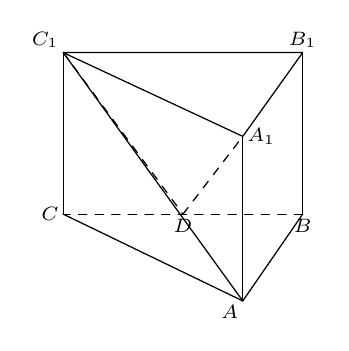
\begin{tikzpicture}[
  x=0.76cm,y=0.76cm,line width=0.45pt,line cap=round,line join=round,
  every node/.style={font=\scriptsize,inner sep=1.5pt}
]
  \coordinate (C)  at (0,1.45);
  \coordinate (B)  at (4.0,1.45);
  \coordinate (D)  at (2.0,1.45);
  \coordinate (A)  at (3.0,0);
  \coordinate (C1) at (0,4.15);
  \coordinate (B1) at (4.0,4.15);
  \coordinate (A1) at (3.0,2.75);

  % Prism edges; BC and the source-indicated interior lines use dashed strokes.
  \draw (C)--(A)--(B);
  \draw[dashed] (B)--(C);
  \draw (C1)--(B1)--(A1)--cycle;
  \draw (C)--(C1) (B)--(B1) (A)--(A1);
  \draw (C1)--(A);
  \draw[dashed] (C1)--(D) (D)--(A1);

  \node[below left] at (A) {$A$};
  \node[below] at (B) {$B$};
  \node[left] at (C) {$C$};
  \node[below] at (D) {$D$};
  \node[right] at (A1) {$A_1$};
  \node[above] at (B1) {$B_1$};
  \node[above left] at (C1) {$C_1$};
\end{tikzpicture}
\end{center}
\nopagebreak[4]
\Needspace{0.4\textheight}
\end{question}
\begin{question}
\gkti{18}
\begin{gktip}
原页记号疑点（待核）：首句称椭圆顶点为 \(A_1,A_2\)，后文使用 \(OA\)、\(A_1P\)、\(AP_1\)；原图左顶点标为 \(A_1(-5,0)\)，右顶点标为 \(A(5,0)\)，没有标出 \(A_2\)。题干与图中的顶点字母不统一。本稿保留题干原字和图中原标记，不将 \(A\) 静默改成 \(A_2\)。
\end{gktip}

如图，\(A_1,A_2\) 为椭圆的两个顶点，\(F_1,F_2\) 为椭圆的两个焦点。

(1) 写出椭圆的方程及准线方程；

\Needspace{5\baselineskip}
(2) 过线段 \(OA\) 上异于 \(O,A\) 的任一点 \(K\) 作 \(OA\) 的垂线，交椭圆于 \(P,P_1\) 两点，直线 \(A_1P\) 与 \(AP_1\) 交于点 \(M\)。求证：点 \(M\) 在双曲线
\nopagebreak[4]
\[
\frac{x^2}{25}-\frac{y^2}{9}=1
\]
上。
\nopagebreak[4]
\begin{center}% Generator: hand-authored TikZ schematic traced from the fixed source; preserve the printed vertex labels verbatim.
% Source ID: src-dcc6a2c21c7b8e7b8f23f5188f34d7f542f94e40f4219b54cfb85a0d7004bc0f
% PDF SHA-256: 7fc0fd289fc486a0ae1c16a9ab5b4f0561830897df6e8897c50666f03d511913
% PDF page 2; printed page 127; question 18.
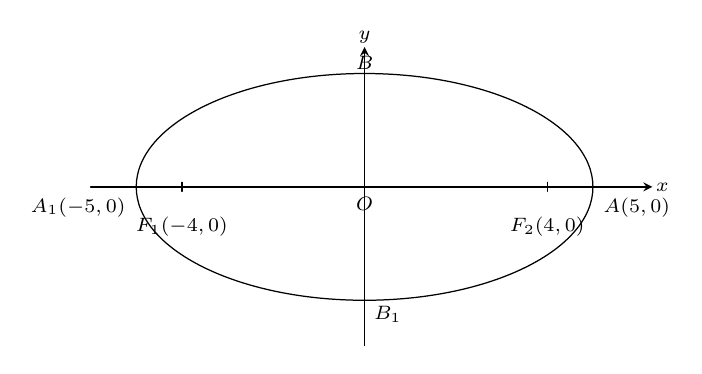
\begin{tikzpicture}[
  x=0.58cm,y=0.48cm,line width=0.45pt,line cap=round,>=stealth,
  every node/.style={font=\scriptsize,inner sep=1.2pt}
]
  \draw[->] (-6.0,0)--(6.3,0) node[right] {$x$};
  \draw[->] (0,-4.2)--(0,3.7) node[above] {$y$};
  \draw (0,0) ellipse [x radius=5,y radius=3];
  \draw (-4,-0.12)--(-4,0.12) (4,-0.12)--(4,0.12);

  % Coordinate labels match the source figure, including its A/A_2 inconsistency.
  \node[below left] at (-5.15,-0.18) {$A_1(-5,0)$};
  \node[below] at (-4,-0.7) {$F_1(-4,0)$};
  \node[below] at (0,-0.18) {$O$};
  \node[below] at (4,-0.7) {$F_2(4,0)$};
  \node[below right] at (5.15,-0.18) {$A(5,0)$};
  \node[above] at (0,3) {$B$};
  \node[below right] at (0.12,-3.05) {$B_1$};
\end{tikzpicture}
\end{center}
\nopagebreak[4]
\Needspace{0.4\textheight}
\end{question}
\begin{question}
\gkti{19}
有三个新兴城镇，分别位于 \(A,B,C\) 三点处，且 \(AB=AC=13\text{ km}\)，\(BC=10\text{ km}\)。今计划合建一个中心医院，为同时方便三镇，准备建在 \(BC\) 的垂直平分线上的 \(P\) 点处。（建立坐标系如图）

(1) 若希望点 \(P\) 到三镇距离的平方和为最小，点 \(P\) 应位于何处？

(2) 若希望点 \(P\) 到三镇的最远距离为最小，点 \(P\) 应位于何处？
\nopagebreak[4]
\begin{center}% Generator: hand-authored TikZ schematic traced from the fixed source; triangle proportions are illustrative.
% Source ID: src-dcc6a2c21c7b8e7b8f23f5188f34d7f542f94e40f4219b54cfb85a0d7004bc0f
% PDF SHA-256: 7fc0fd289fc486a0ae1c16a9ab5b4f0561830897df6e8897c50666f03d511913
% PDF page 2; printed page 127; question 19.
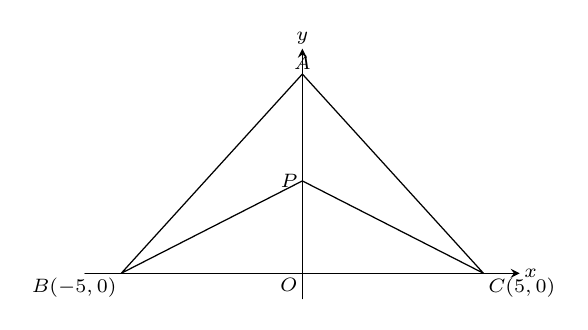
\begin{tikzpicture}[
  x=0.46cm,y=0.46cm,line width=0.45pt,line cap=round,>=stealth,
  every node/.style={font=\scriptsize,inner sep=1.5pt}
]
  \coordinate (O) at (0,0);
  \coordinate (A) at (0,5.5);
  \coordinate (P) at (0,2.55);
  \coordinate (B) at (-5,0);
  \coordinate (C) at (5,0);

  \draw[->] (-6.0,0)--(6.0,0) node[right] {$x$};
  \draw[->] (0,-0.7)--(0,6.2) node[above] {$y$};
  \draw (A)--(B) (A)--(C) (P)--(B) (P)--(C);

  \node[above] at (A) {$A$};
  \node[below left] at (B) {$B(-5,0)$};
  \node[below right] at (C) {$C(5,0)$};
  \node[below left] at (O) {$O$};
  \node[left] at (P) {$P$};
\end{tikzpicture}
\end{center}
\nopagebreak[4]
\end{question}
\begingroup
\renewenvironment{question}{\Needspace{0.25\textheight}}{}
\begin{question}
\gkti{20}

设 \(y=f(x)\) 是定义在区间 \([-1,1]\) 上的函数，且满足条件：

① \(f(-1)=f(1)=0\)；

② 对任意的 \(u,v\in[-1,1]\)，都有 \(|f(u)-f(v)|\leq|u-v|\)。

(1) 证明：对任意的 \(x\in[-1,1]\)，\(x-1\leq f(x)\leq1-x\)；

\Needspace{5\baselineskip}
(2) 判断函数
\nopagebreak[4]
\[
g(x)=\begin{cases}
1+x,&x\in[-1,0),\\
1-x,&x\in[0,1],
\end{cases}
\]
是否满足题设条件；

(3) 在区间 \([-1,1]\) 上是否存在满足题设条件的函数 \(y=f(x)\)，且使得对任意的 \(u,v\in[-1,1]\)，都有 \(|f(u)-f(v)|=u-v\)，若存在，请举一例；若不存在，请说明理由。

\end{question}
\endgroup